\section{Algorithm} \label{GLOBALsec:computation}

\renewcommand\theenumi{\algletter\arabic{enumi}}
\renewcommand\labelenumi{{\rmfamily \algletter\arabic{enumi}.}}
\setlength{\leftmargini}{2em}

The algorithm we present here computes the shortest path in the alignment graph
using a variant of \A that handles pruning (\cref{GLOBALsec:astar}). This
depends on the efficient computation of the heuristics
(\cref{GLOBALsec:compute-sh,GLOBALsec:compute-csh}). \cref{GLOBALsec:impl}
contains further implementation notes.

At a high level, we first initialize the heuristic by finding all seeds and
matches and precomputing the potential $P[i]$ and layers $\layer_\ell$. Then we
run the \A search that evaluates the heuristic in many states, and updates the
heuristic whenever a match is pruned.

\subsection{Computing the \sh} \label{GLOBALsec:compute-sh}

We compute the \sh using an array $LS$
that contains for each layer $\layer_\ell$ the \emph{layer
start} $LS[\ell] := i_\ell = \max \{i : \shscore\st i\cdot \geq \ell\}$.

We give the algorithms to precompute $LS$, to evaluate the
heuristic using it, and to update it after pruning.

\paragraph{Precomputation}
\begin{samepage}
\newcommand{\algletter}{R}
\begin{enumerate}
  \item Compute the set of seeds $\seeds$ by splitting $A$ into consecutive kmers.
  \item Build a hashmap containing all kmers of $B$.
  \item For each seed, find all matches via a lookup in the hashmap.
        In case of inexact matches ($r=2$), all
        sequences at distance $1$ from each seed are looked up independently.
        The matches $\matches$ are stored in a hashmap keyed by the start
        of each match.
  \item Initialize the array of potentials $P$ by iterating over the seeds backwards.
  \item Initialize the array of layer starts $LS$ by setting $LS[0] = n$ and iterating over the
        seeds backwards. For each seed $s=\substr Ai{i'}$ that has matches,
        push $\seedscore(s)$ copies of $i$ to the end of
        $LS$.
\end{enumerate}
\end{samepage}

\paragraph{Evaluating the heuristic in $u = \st ij$}
\begin{samepage}
\newcommand{\algletter}{E}
\begin{enumerate}
  \item Look up the potential $P[i]$.
  \item \label{GLOBALstep:bin-search} $\shscore(u) {=} \max \{\ell : LS[\ell] \geq i\}$ is found by a binary search over $\ell$.
  \item Return $h(u) = P[i] - \shscore(u)$.
\end{enumerate}
\end{samepage}

\paragraph{Pruning when expanding match start $u = \st ij$}
\begin{samepage}
\newcommand{\algletter}{P}
\begin{enumerate}
  \item Compute $seedscore_{old} := \seedscore(s)$ and
        $\ell_{old} := \shscore(u)$.
  \item Remove all matches from $\matches$ that start at $u$.
  \item Compute $seedscore_{new} := \seedscore(s)$ and
        set $\ell_{new} := \ell_{old} - seedscore_{old} + seedscore_{new}$.
        If $\ell_{new} < \ell_{old}$,
        remove layers $LS[\ell_{new}+1]$ to
        $LS[\ell_{old}]$ from $LS$ and shift down larger elements $LS[\ell]$
        with $\ell > \ell_{old}$ correspondingly.
        %This effectively decreases $\shscore\st {i'}{j'}$ by
        %$\ell_{old}-\ell_{new}$ for all $i' \leq i$.
\end{enumerate}
\end{samepage}

\subsection{Computing the \csh} \label{GLOBALsec:compute-csh}

The computation of the \csh is similar to that of the \sh. It involves a
slightly more complicated array $LM$ of \emph{layer matches} that associates to
each layer $\layer_\ell$ a list of matches with score $\ell$:
$LM[\ell] = \{m\in \matches \,|\, \chainscore(m) = \ell\}$.  The score
$\cshscore(u)$ is then the largest $\ell$ such that $LM[\ell]$ contains a match
$m$ preceded by $u$.

Our algorithm for computing the \csh is similar to the one for the
\sh~(\cref{GLOBALsec:compute-sh}). Hence we highlight only the steps which differ (\eg
step 2$'$ is used instead of 2 for the \sh).

\paragraph{Precomputation}
\renewcommand\theenumi{\algletter\arabic{enumi}$'$}
\renewcommand\labelenumi{{\rmfamily \algletter\arabic{enumi}$'$.}}
\setlength{\leftmargini}{2.3em}
\begin{samepage}
\newcommand{\algletter}{R}
\begin{enumerate}
  \addtocounter{enumi}{4} % skip 1-4
  \item Initialize $LM$ by setting $LM[0] = \emptyset$. Iterate over all
        matches in order of decreasing $i$ of the match start, compute
        $\ell=\chainscore(m)$ (see point 2$'$ below), and add $m$ to $LM[\ell]$.
\end{enumerate}
\end{samepage}

\paragraph{Evaluating the heuristic in $u = \st ij$}
\begin{samepage}
\newcommand{\algletter}{E}
\begin{enumerate}
  \addtocounter{enumi}{1} % skip 1
  \item Because of \cref{GLOBALlem:contour}, the score $\cshscore(u)$
        can be computed using binary search: $\cshscore(u) \geq \ell$ holds if
        and only if one of the layers $LM[\ell']$ with ${\ell\leq \ell'<\ell+r}$
        contains a match $m$ with $u\preceq m$. This is checked by simply iterating over
        all the matches in these layers.
\end{enumerate}
\end{samepage}

\paragraph{Pruning when expanding match start $u = \st ij$}
\newcommand{\algletter}{P}
\begin{enumerate}
  \addtocounter{enumi}{1} % skip 1
  \item Compute $\ell_u=\cshscore(u)$, and remove all matches that start at $u$
        from layers $LM[\ell_u - r+1]$ to $LM[\ell_u]$.
  \item Iterate over increasing $\ell$ starting at $\ell=\ell_u+1$ and
        recompute $\ell':=\chainscore(m)\leq \ell$ for all matches $m$ in
        $LM[\ell]$. Move $m$ from $LM[\ell]$ to layer $LM[\ell']$ whenever
        $\ell' \neq \ell$. Stop when either $r$ consecutive layers are
        unchanged, in which case no further changes of $\chainscore(m)$ can
        happen because of \cref{GLOBALeq:chainscore} and $\matchscore(m) \leq r$, or
        when all matches in $r$ consecutive layers have shifted down by the same
        amount, say ${\Delta := \ell-\ell'}$. In the latter case,
        $\chainscore(m)$ decreases by $\Delta$ for all matches with score at
        least $\ell$. We remove the emptied layers ${LM[\ell-\Delta+1]}$ to
        $LM[\ell]$ so that all higher layers shift down by $\Delta$.
\end{enumerate}

% Forward include so these appear before the Results section.

\subsection{Implementation \astarix}

Our \astarix implementation uses an adjacency list graph data structure to
represent the reference and the trie in a unified way, representing each letter
by a separate edge object.
%\para{Reverse Complement Alignment}
To represent the reverse complementary walks in $\RG$, the vertices are doubled,
connected in the opposite direction, and labeled with complementary nucleotides
($\texttt{A} \leftrightarrow \texttt{T}$, $\texttt{C} \leftrightarrow
\texttt{G}$).
%
%\para{Default Parameters}
We do not limit the number of memoized heuristic function values
(\cref{TRIEpara:memoization}), but note we could do so by resetting the memoization
table periodically.
%
Our implementation of \dijkstra reuses the same \astarix codebase except the
use of a heuristic function (\ie, with $h \equiv 0$).
\begin{figure}[H]
  \centering
  \subfloat[$e{=}1\%$, exact matching]{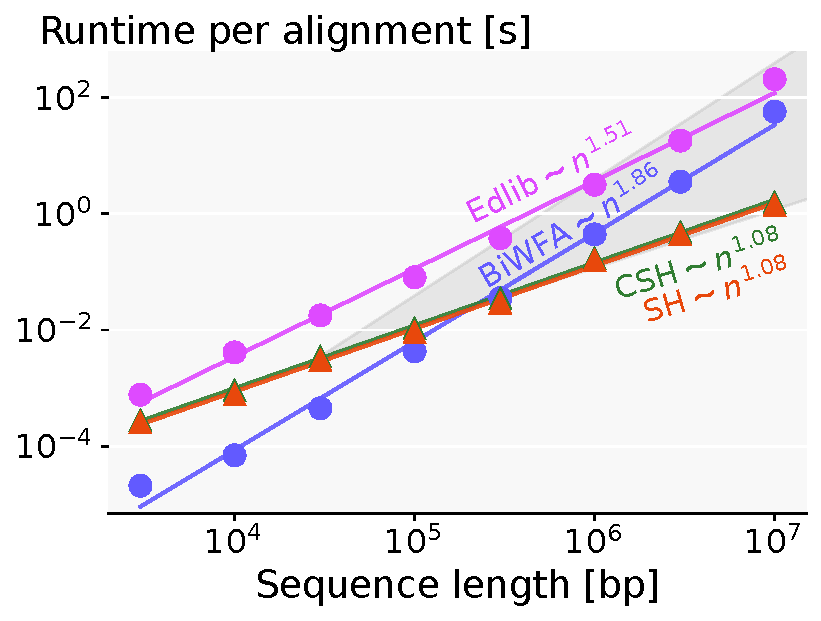
\includegraphics[width=0.4\linewidth]{imgs/fig4/tools_e0.01_labels.pdf}
  \label{GLOBALfig:scaling-n-1}}
  %\hfill
  \subfloat[$e{=}5\%$, exact matching]{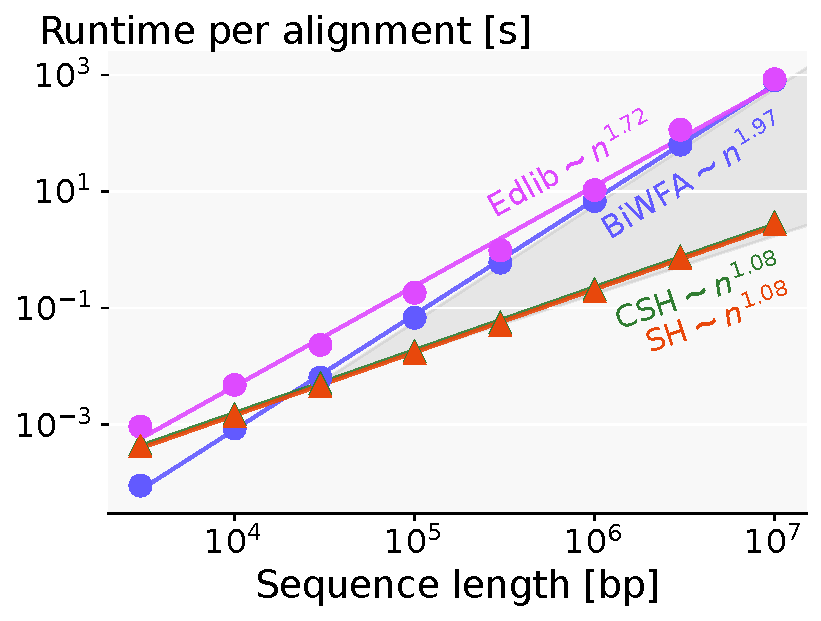
\includegraphics[width=0.4\linewidth]{imgs/fig4/tools_e0.05_labels.pdf}
  \label{GLOBALfig:scaling-n-5}}\\
  %\hfill
  \subfloat[$e{=}10\%$, inexact matching]{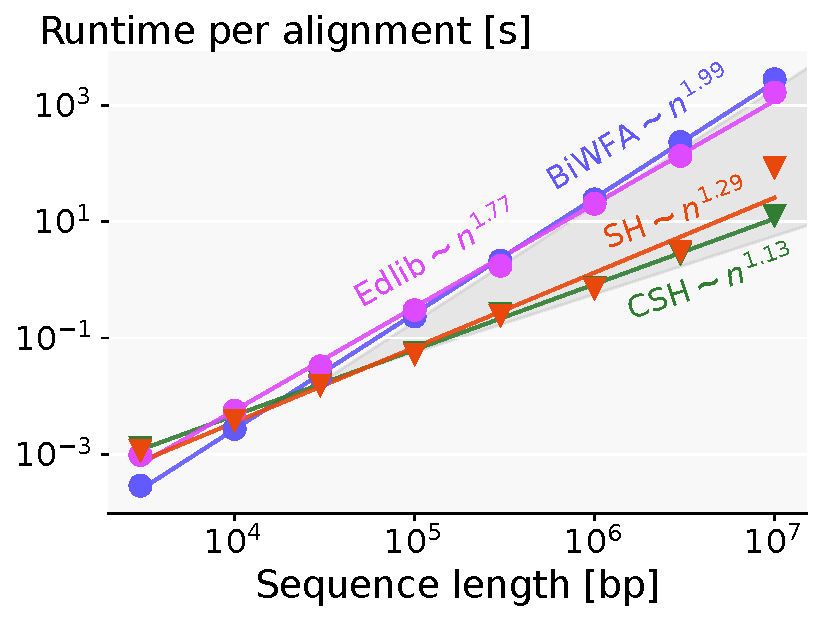
\includegraphics[width=0.4\linewidth]{imgs/fig4/tools_e0.1_labels.pdf}
  \label{GLOBALfig:scaling-n-10}}
  %\hfill
  \subfloat[$e{=}15\%$, inexact matching]{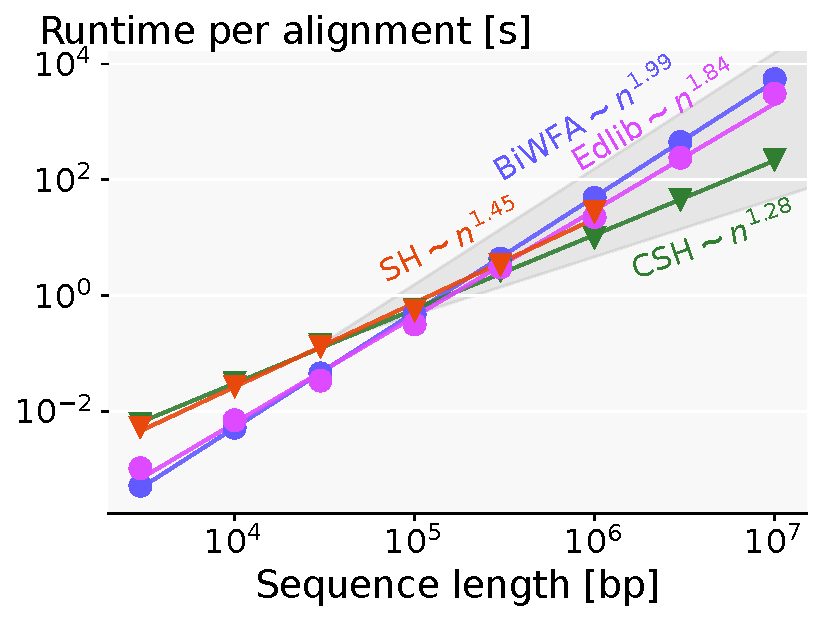
\includegraphics[width=0.4\linewidth]{imgs/fig4/tools_e0.15_labels.pdf}
  \label{GLOBALfig:scaling-n-15}}

  \caption[Runtime scaling with sequence length (multiple error rates)]{Log-log
    plots of the runtime for aligning \textbf{synthetic sequences} of increasing
    length for \astarpa \sh~(\SH), \astarpa \csh~(\CSH), \edlib~(\edlibsymbol)
    and \wfa~(\wfasymbol). The slopes of the bottom (top) of the dark-grey cones
    correspond to linear (quadratic) growth. For $e{\leq} 5\%$,
    \SH~(\shsymbolsq) and \CSH~(\cshsymbolsq) use $k{=}15$, $r{=}1$. For $e{\ge}
    10\%$, \SH~(\shsymbol) and \CSH~(\cshsymbol) use $k{=}15$, $r{=}2$. The
    missing data points for \SH at $e{=}15\%$ are due to exceeding the memory
    limit ($\qty{30}{GB}$). Each runtime is the average over $\lfloor 10^7 / n
    \rfloor$ alignments.}
  \label{GLOBALfig:scaling-n}
\end{figure}


\renewcommand\theenumi{\arabic{enumi}}
\renewcommand\labelenumi{{\rmfamily \arabic{enumi}.}}
\setlength{\leftmargini}{3mm}
